\documentclass[10pt]{article}
\usepackage[a4paper,left=2.54cm,top=2.54cm,right=2.54cm,bottom=2.54cm]{geometry}
\usepackage{fancyhdr}
\setlength{\headsep}{1.40cm} % Adjust the space after the header
\usepackage{afterpage}
\usepackage{setspace}
\usepackage{iccfdTemplate/bibspacing} 
\singlespacing

%%%% YOU CAN PUT YOUR OWN DEFINITIONS HERE
\newfont{\toto}{msbm10 at 12 pt}
\newfont{\ithd}{cmr9}

\newcommand{\si}[1]{\rm\scriptscriptstyle{#1}}
%%%% END OF YOUR DEFINITIONS 
 
\pagestyle{fancyplain}
\renewcommand{\headrulewidth}{0pt}

\usepackage{amsmath,amsthm,amsfonts,amssymb}
\usepackage[pdftex]{graphicx} 
\usepackage[T1]{fontenc}

%%! Additional usepackage
\usepackage{physics} 
\usepackage{hyperref} 
\hypersetup{
    colorlinks=true,
    linkcolor=blue,
    filecolor=magenta,      
    urlcolor=cyan,
    }
\usepackage{subcaption}

%%%% CONFERENCE HEADER. REPLACE xxxx WITH 4-DIGIT PAPER NUMBER ASSIGNED BY CONFERENCE COMMITTEE.

% \rhead{\ithd{\bf ICCFD12-2024-xxxx\\  \   \\}}
\lhead{\ithd{\bf Twelfth International Conference on \\      
Computational Fluid Dynamics (ICCFD12), \\
Kobe, Japan, July 14-19, 2024
}}
% Define the left and center headers to be empty or contain fixed content
\rhead{}
\chead{}

\usepackage{titling}
\setlength{\droptitle}{0em}  
\pretitle{\vspace{-4em}\begin{center}\LARGE}
\posttitle{\end{center}\vspace{-1em}}
\preauthor{\begin{center}\large}
\postauthor{\end{center}\vspace{-3em}}


\title{
\bf Positivity-preserving algorithm for implicit finite
volume methods simulating compressible flows
}
\author{
Qian Wang$^{*}$, Hanyu Zhou$^{**}$\\
Corresponding author: Email@email.email \\
$^{*}$ Beijing Computational Science Research Center, Beijing, 100088, China.\\
$^{**}$ Department of Engineering Mechanices, Tsinghua Universiy, Beijing, 100084, China.
}
\date{}

\begin{document}

%%%% TITLE
\maketitle
\afterpage{\fancyhead{}}

%%%% ABSTRACT AND KEYWORDS
%\vskip0.5cm
\centerline{
\begin{minipage}[t]{150mm}
{\bf Abstract:} 
The body of your abstract belongs here. ICCFD is the outcome of the merger of two important CFD conferences: the International Conference on Numerical Methods in Fluid Dynamics, ICNMFD (since 1969) and International Symposium on Computational Fluid Dynamics, ISCFD (since 1985). The first ICCFD conference was held in 2000 in Kyoto, the second in 2002 in Sydney, the third in 2004 in Toronto, the fourth in 2006 in Ghent, the fifth in 2008 in Seoul, the sixth in 2010 in St Petersburg, the seventh in Hawaii in 2012, the eighth in Chengdu in 2014, the ninth in Istanbul in 2016, the tenth in Barcelona in 2018, and the Eleventh in Hawaii in 2022. The Twelfth conference, ICCFD12 will be held on the Kobe, Japan in July 2024.
\vskip0.2cm
{\it Keywords:} Numerical Algorithms, Computational Fluid Dynamics, Turbulence Modeling, Aeroacoustics. \\
\end{minipage}
}
\vskip0.5cm

%%%% MAIN PART
% \section{Introduction}
% This is the main part of the paper. Its length should be no longer than {\bf 25 pages}, including key figures and references. 
% It can be divided in as many sections as you decide. The paper must be prepared using this template 
% and compiled using standard \LaTeX, generating a {\bf PDF file} that will be finally uploaded. If
% another kind of word processor is utilized, please adhere to the formatting provided in the PDF template.


% \section{Problem Statement}
% This document allows you to easily include references \cite{book,journalpaper}, equations, figures (see Figure \ref{fig:logo}) or anything else you
% desire into a clean and compact environment of \LaTeX.  For example if you'd like to impress a date you can write
% the unsteady heat equation as
% \begin{eqnarray}
% \frac{\partial \mathbf{V}}{\partial t} - \alpha \left( \frac{\partial^2 \mathbf{V}}{\partial x^2} +
%        \frac{\partial^2 \mathbf{V}}{\partial y^2} +
%        \frac{\partial^2 \mathbf{V}}{\partial z^2} \right)
% = 0
% \label{eq:heat}
% \end{eqnarray}
% where $x, y, z$ are the space dimensions and $\alpha$ is a parameter.  If you felt inclined you could define $\mathbf{V}$ as
% %
% $$\mathbf{V} = y^2 z - \text{cos}(0.1 x)$$
% %
% for a non-exact solution.  Computational fluid dynamics~\cite{paper} can be used to discretize the equations, apply boundary conditions and 
% simulation the unsteady nature of the flow.  An innovative method to simulate the heat equation could even be submitted to ICCFD12.

%   The scope of ICCFD12~\cite{web} is devoted to all innovative aspects of CFD, basic and applied.  Subjects of interest include but are not limited
% to: 
% \begin{itemize}

%     \item Innovative algorithm development for flow simulations: higher-order methods, iterative methods, parallel
%           algorithms, mesh adaptation, grid generation, meshless methods, immersed boundary methods and level-set
%           methods. 
          
%     \item Advances in modeling of flow physics in the area of: steady and unsteady flows, compressible and incompressible 
%           flows, flows in porous media, hypersonic and reacting flows, turbulence (transition, DNS/LES, etc.), multi-phase 
%           flows, boundary layer stability and vortex dynamics. 
          
%     \item Advanced multidisciplinary applications using the above mentioned technologies: aeroacoustics, flow
%           control, biomedical fluid mechanics, large scale applications, verification and validation methods, and
%           turbomachinery. 
          
% \end{itemize}

% \begin{figure}[t]
%   \centering 
%   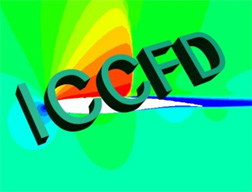
\includegraphics[height=2.0in]{iccfdTemplate/exampleFigure.jpg}
%   \caption{This is the logo of ICCFD.}
%   \label{fig:logo}
% \end{figure}


% \subsection{Subsection Title Example}


% \subsubsection{Sub-subsection Title Example}


% \section{Conclusion and Future Work}
% ICCFD12 will be held at the Kobe international conference center in Port Island, Kobe, Japan. We look forward to welcoming you all to what we hope will be a memorable event.



% !TeX root = ./PPRobustDraft_ICCFD.tex


\section{Introduction}
\label{sec:intro}


\section{Implicit Finite Volume Method}
\label{sec:CFV}

\newcommand{\trans}{^\mathrm{T}}
\newcommand{\U}{\mathbf{U}}
\newcommand{\F}{\mathbf{F}}
\newcommand{\x}{\mathbf{x}}
\newcommand{\OO}{\mathbf{\Omega}}
\newcommand{\UM}{\overline{\U}}
\newcommand{\Fn}{\tilde{\F}}
\newcommand{\n}{\mathbf{n}}
\newcommand{\uu}{\overline{\mathbf{U}}}
\newcommand{\R}{\mathbf{R}}
\newcommand{\inc}{\mathrm\Delta}
\newcommand{\Tau}{\mathrm{T}}
\renewcommand{\real}{\mathrm{Re}}
\newcommand{\imag}{\mathrm{Im}}

\newcommand{\CFLt}{\text{CFL}_t}
\newcommand{\CFLtau}{\text{CFL}_\tau}

\newcommand{\eeqref}[1]{Eq.\eqref{#1}}
\newcommand{\um}{\overline{u}}
\newcommand{\us}{\mathbf{u}}
\newcommand{\SAll}{\mathcal{S}}

\newcommand{\FF}{\mathcal{F}}

\newcommand{\eye}{\mathbf{I}}

\subsection{Governing Equations}
\label{ssec:GovEq}

The compressible Navier-Stokes equations are
written in the conservative form:
\begin{equation}
    \label{eq:NS}
    \frac{\partial \U}{\partial t} +
    (\F - \F_v) \cdot \mathbf\nabla = 0
\end{equation}
where $\U$ is the vector of conservative quantities and
$\F=[\F_1,\F_2,\F_3]$,
$\F_v=[\F_{v,1},\F_{v,2},\F_{v,3}]$
are
inviscid and viscous tensors of
their flux.
The $\nabla$ is the spacial derivative operator, and for
some 3-D vector field $\mathbf{v}$, $\mathbf{v}\trans \cdot \nabla$
is the divergence of the vector field.
In cartesian coordinates $x_k, k=1,2,3$, the components of
the conservative quantities and the flux terms are
\begin{equation}
    \U = \begin{bmatrix}
        \rho \\ \rho u_1 \\ \rho u_2 \\ \rho u_3 \\ E
    \end{bmatrix},\ \
    \F_j = \begin{bmatrix}
        \rho u_j                   \\
        \rho u_1u_j + p\delta_{1j} \\
        \rho u_2u_j + p\delta_{2j} \\
        \rho u_3u_j + p\delta_{3j} \\
        (E+p)u_j                   \\
    \end{bmatrix},\ \
    \F_{v,j} = \begin{bmatrix}
        0                                \\
        \tau_{1j}                        \\
        \tau_{2j}                        \\
        \tau_{3j}                        \\
        \sum_{k=1}^3{u_k\tau_{kj}} - K_j \\
    \end{bmatrix}
\end{equation}
where $\rho$ is density,
$u_i, i=1,2,3$ are velocity components,
$p$ is pressure,
$E$ is total energy per unit volume,
$\tau_{ij}, i,j=1,2,3$ are viscous stress tensor components
and
$K_i, i=1,2,3$ are heat flux components.
$\delta_{ij}$ is
Kronecker delta.
With ideal gas equation of state and energy equation:
\begin{equation}
    \begin{aligned}
        E & = e + \frac{1}{2}\rho\sum_{k=1}^{3}(u_ku_k) \\
        p & =\rho R_g T                                 \\
        e & = \frac{p}{\gamma - 1}
    \end{aligned}
\end{equation}
and Newtonian viscosity and Fourier
heat conduction relations:
\begin{equation}
    \begin{aligned}
        \\
        \tau_{ij} & =
        \mu\left(\frac{\partial u_i}{\partial x_j} + \frac{\partial u_j}{\partial x_i}\right)
        -
        \frac{2}{3}\mu \delta_{ij}\sum_{k=1}^{3}{\frac{\partial u_k}{\partial x_k}} \\
        K_i       & = - \kappa \frac{\partial T}{\partial x_i}
    \end{aligned}
\end{equation}
the N-S equations are closed.
In the relations above, $T$ is temperature,
$\gamma$ is specific heat ratio, $e$ is internal energy,
$R_g$ is  gas constant, $\mu$ is dynamic viscosity,
$\kappa$ is thermal conductivity.
Specific heat ratio $\gamma$ is $1.4$ in this paper unless specified
otherwise.
The current paper only
considers using the gas property $\kappa = \mu c_p / Pr$,
and $\mu=\mu_{\infty}$ being a constant,
while $c_p$ is special heat capacity
at constant pressure and
Prandtl number $Pr$ is fixed to 0.71 in this paper.
When $\mu=0$,
$\F_v=0$ and
equation \eqref{eq:NS} reduces to
the inviscid Euler equation.
Two-dimensional and one-dimensional forms of the N-S equations
can be easily derived.

\subsection{High-order Finite Volume Spacial Discretization}
\label{ssec:FV}




This subsection provides a general framework of
finite volume discretization.
The computational domain $\OO$ is divided
into $N_{cell}$ cells $\OO_i, i=1,2,...N_{cell}$ which
are non-overlapping while $\cup_i{\OO_i} = \OO$,
forming an unstructured mesh.
An averaging operation of conservative quantities
over each cell is defined as
\begin{equation}
    \label{eq:FVMean}
    \UM_i = \frac{1}{\overline{\OO}_i}\int_{\OO_i}\U(\x)\dd \Omega
\end{equation}
where $\overline{\OO}_i$ is the volume of $\OO_i$.

Next, a degree $k$ piecewise polynomial reconstruction is
obtained to approximate the distribution of
quantities within each cell:
\begin{equation}
    \label{eq:FVRec}
    \U_i(\x) = \UM_i + \sum_{l=1}^{\mathrm{NDOF}(k)}{\U_i^l\varphi_{i,l}(\x) }
\end{equation}
in which
$\U_j(\x)$ is the local polynomial distribution on cell $j$,
and
$\varphi_{j,i}(\x)$ are
polynomial basis functions.
\eeqref{eq:FVRec} can be reformed as a scalar field reconstruction
\begin{equation}
    \label{eq:FVRecScalar}
    u_i(\x) = \overline{u}_i + \sum_{l=1}^{\mathrm{NDOF}(k)}{u_i^l\varphi_{i,l}(\x) }
\end{equation}
where $u_i(\x)$ is one of $\rho(\x), \rho u_1(\x)\dots$.
The quantity reconstructed $u_i$ should not
be confused with the velocity components $u_1, u_2, u_3$ in the context of
reconstruction.

There are $\mathrm{NDOF}(k)$ polynomial bases for reconstruction on
each cell.
The current paper uses zero-mean Taylor basis
for reconstruction \cite{wang2017compact_VR}, therefore
for 2-D reconstruction, $\mathrm{NDOF}(k) = (k+2)(k+1)/2 -1$.
Given a specific reconstruction method,
the reconstruction coefficients $\U_i^l$ or to say $u_i^l$
can be determined using
the distribution of mean values $\UM_i, i=1,2...N_{cell}$
(or
$\um_i, i=1,2...N_{cell}$ as components)
along with boundary conditions.

With the piecewise polynomial approximation,
the PDEs \eqref{eq:NS} can therefore become ODEs
with cell averaging applied
\begin{equation}
    \label{eq:FVInt}
    \frac{\dd\UM_i}{\dd t}
    +\sum_{j\in S_i, j\neq i}{\left(
        \int_{f_{ij}}{
            [\Fn(\U_i,\U_j) - \Fn_v(\U_i,\U_j, \nabla \U_i, \nabla \U_j)] \cdot \n  \dd A
        }\right)
    }
    = 0
\end{equation}
where $\Fn(\U_i,\U_j)$ and $\Fn_v(\U_i,\U_j, \nabla \U_i, \nabla \U_j)$ are approximations
of exact fluxes on the cell interfaces,
and $f_{ij}=\OO_i \cap \OO_j$ is the interface between $i,j$ cells.
Set $S_i$ denotes the compact stencil of cell $i$.
Because the piecewise polynomial approximation \eqref{eq:FVRec} does not
guarantee a continuous distribution on interfaces,
the numerical fluxes
$\Fn(\U_i,\U_j)$, $\Fn_v(\U_i,\U_j, \nabla \U_i, \nabla \U_j)$ are
functions of the approximate field on both sides.
Inviscid numerical
flux $\Fn(\U_i,\U_j)$ is typically an approximate Riemann solver,
and the current paper uses the local Lax-Friedrichs flux.
Numerical viscous flux $\Fn_v(\U_i,\U_j, \nabla \U_i, \nabla \U_j)$
in this paper follows the practice of Wang \cite{wang2017compact_VR},
which uses a dGRP type of penalty term in the viscous flux.
The integration of flux terms on the cell interfaces
are conducted using numerical quadrature rules with
enough algebraic precision.

\eeqref{eq:FVInt}
is referred to as the semi-discretized form of finite volume method,
because it does not include spacial derivatives.
The inviscid term has a truncation error of $O(h^{k+1})$ for smooth problems,
with $h$ being the size of cell.
As the approximate polynomial representations $\U_i$ are determined
by average values $\UM_i$, \eqref{eq:FVInt} can be rearranged into
\begin{equation}
    \label{eq:FVODECell}
    \derivative{\uu_i}{t} = \R_i(t, [\uu_j, j\in\SAll_i])
\end{equation}
and
\begin{equation}
    \R_i(t, [\uu_j, j\in\SAll_i]) = -\sum_{j\in S_i, j\neq i}{\left(
        \int_{f_{ij}}{
            [\Fn(\U_i,\U_j) - \Fn_v(\U_i,\U_j, \nabla \U_i, \nabla \U_j)] \cdot \n  \dd A
        }\right)
    }
\end{equation}
where
$\SAll_i$ is the set of cells that the right-hand side of cell $i$ is
dependent on. The arguments in the numerical flux functions are omitted.
Note that $\SAll_i$ is generally a superset of $\S_i$ due to
the reconstruction process.
The
assembled form of \eeqref{eq:FVODECell} can be denoted as
\begin{equation}
    \label{eq:FVODE}
    \derivative{\uu}{t} = \R(t, \uu)
\end{equation}
with
\begin{equation}
    \uu = \begin{bmatrix}
        \UM_1 \\
        \dots \\
        \UM_{N_{cell}}
    \end{bmatrix},\ \
    \R = \begin{bmatrix}
        -\sum_{j\in S_1, j\neq 1}{\left(
            \int_{f_{1,j}}{
                [\Fn - \Fn_v] \cdot \n  \dd A
            }\right)
        }     \\
        \dots \\
        -\sum_{j\in S_{N_{cell}}, j\neq N_{cell}}{\left(
            \int_{f_{N_{cell},j}}{
                [\Fn - \Fn_v] \cdot \n  \dd A
            }\right)
        }
    \end{bmatrix}
\end{equation}





\subsection{Variational Reconstruction}
\label{ssec:VR}
In order to determine the coefficients of polynomial bases $\U_i^l$ (or $u_i^l$ for each scalar) in
\eeqref{eq:FVRec}, a reconstruction method needs to be specified.
Traditional 2nd order FV methods for unstructured grid
needs only to reconstruct a $k=1$ polynomial, namely linear
distribution on each cell.
The variational reconstruction \cite{wang2017compact_VR}
is a compact high-order
reconstruction scheme, and it achieves high-order
accuracy on a compact stencil.
The current section will explain the variational reconstruction briefly
and specify details concerning following numerical tests.

The current paper uses local zero-mean Taylor basis, similar to
\cite{wang2017compact_VR}.
Taking 2 dimensional polynomials as an example:
\begin{equation}
    \begin{aligned}
        \varphi_{i,l} & =
        \left(\frac{x - x_{c,i}}{\inc x_i}\right)^{p_l}
        \left(\frac{y - y_{c,i}}{\inc y_i}\right)^{q_l}
        -
        \overline{
            \left(\frac{x - x_{c,i}}{\inc x_i}\right)^{p_l}
            \left(\frac{y - y_{c,i}}{\inc y_i}\right)^{q_l}
        }
    \end{aligned}
\end{equation}
where $[x_{c,j},y_{c,j}]\trans = \x_{c,j}$ are barycenters of cell $j$,
$\inc x_i,\inc y_i$ are the cell's length scale, and $p_l,q_l$ are
powers of the bases. If 2-D $k=3$ basis is used, $p_l=[1,0,2,1,0,3,2,1,0]_l$,
and $q_l=[0,1,0,1,2,0,1,2,3]_l$.
The mean value term makes the basis zero-mean, which is calculated with:
\begin{equation}
    \overline{
        \left(\frac{x - x_{c,i}}{\inc x_i}\right)^{p_l}
        \left(\frac{y - y_{c,i}}{\inc y_i}\right)^{q_l}
    }
    =
    \frac{1}{\overline{\OO}_j}\int_{\OO_j}{
        \left(\frac{x - x_{c,i}}{\inc x_i}\right)^{p_l}
        \left(\frac{y - y_{c,i}}{\inc y_i}\right)^{q_l}
    }\dd \Omega
\end{equation}

The length scales are chosen to be the largest distance of nodes from the
barycenter, which has the from
\begin{equation}
    \inc x_j = \inc y_j = \max_k(\|\x_{j,k} - \x_{c,j}\|_2)
\end{equation}
where $\x_{j,k}$ are coordinates of nodes belonging to cell $j$.
The base functions are scaled to be isotropic in order
to improve the rotational similarity of the base functions
and reduce the stiffness of the reconstruction system.

The variational reconstruction defines the solution of reconstruction coefficients
to be the minimum point of a globally defined functional $I$
\begin{equation}
    I = \sum{I_f}
\end{equation}
where $I_f$ are interface jump integrations (IJI) defined on each cell interface $f$.
Hereafter, we use $f=f_{ij}$ to denote the interface of cell $i$ and $j$ by default.
Using 2-D as an example, the current paper uses IJI in the form of
\begin{equation}
    I_f = \omega_f^G\int_{\OO_i \cap \OO_j}{
        \sum_{p+q=0}^{p + q\leq k}\left[
            \omega_f^D(p,q)
            \left(
            \partialderivative{^{p+q}u_i(x,y)}{x^p\partial y^q}
            -
            \partialderivative{^{p+q}u_j(x,y)}{x^p\partial y^q}
            \right)
            \right]^2
        \dd f
    }
\end{equation}
where $\omega_f^G$ is geometric weight and
$\omega_f^D$ is derivative weight.
The IJI characterizes facial discontinuities of reconstruction polynomials using
the difference of
function values and their various partial derivatives on the interface.
For 2-D simulation and 3rd degree polynomial reconstruction, the current paper uses
\begin{equation}
    \begin{aligned}
        \omega_f^D(0,0) & = 1\times \omega_D(0)                                                                                    \\
        \omega_f^D(1,0) & = \omega_f^D(0,1) = 1\times \omega_D(1)                                                                  \\
        \omega_f^D(2,0) & = \omega_f^D(0,2) = 1\times \omega_D(2),\ \omega_f^D(1,1) = \sqrt{2}\times \omega_D(2)                   \\
        \omega_f^D(3,0) & = \omega_f^D(0,3) = 1\times \omega_D(3),\ \omega_f^D(1,2) = \omega_f^D(2,1) = \sqrt{3}\times \omega_D(3) \\
    \end{aligned}
    \label{eq:wdRotRatio}
\end{equation}
with
\begin{equation}
    \omega_D(0) = 1, \omega_D(1) = 1, \omega_D(2) = \frac{1}{2}, \omega_D(3) = \frac{1}{6}
    \label{eq:wdHQMOPT}
\end{equation}
as the derivative weight.
The derivative weights with their ratios fixed
in \eeqref{eq:wdRotRatio} are rotational invariant and
isotropic.

As the current paper only uses near uniform and isotropic mesh,
geometric weights
$\omega^G_f$ are all set to 1.

The solution to the variational reconstruction system is defined by the minimum problem
\begin{equation}
    u_i^l = \mathop{\arg \min}(I)
\end{equation}
defines.
It is observed that $I$ is a quadratic function of $u_i^l, i = 1...N_{cell}$ and
$I\geq 0$,
therefore $I$ is a positive semi-definite quadratic form about the global vector of reconstruction
coefficients. Consequently, the minimum problem transfers to a linear equation
\begin{equation}
    \partialderivative{I}{u_i^l} = 0, l=1,2,\dots \mathrm{NDOF}(k),\ \ i=1,2,\dots N_{cell}
\end{equation}
This linear equation can be arranged in a cell-wise form:
\begin{equation}
    \label{eq:vrBlockEq}
    \sum_{f=f_{ij},j\in S_i, j\neq i}{ \mathbf{A}_{ij} \us_i}
    =
    \sum_{f=f_{ij},j\in S_i, j\neq i}{ \mathbf{B}_{ij} \us_j + \mathbf{b}_{ij} (\overline{u}_j - \overline{u}_i)}
\end{equation}
where $S_i$ is the compact stencil of $i$ composed of cell $i$ and its face neighbors.
Local reconstruction coefficient vector is $\us_i = [u_i^1,u_i^2\dots]\trans$.
The reconstruction coefficient matrices and vectors in \eeqref{eq:vrBlockEq}
are determined by the form of IJI:
\begin{equation}
    \label{eq:vrCoeffs}
    \begin{aligned}
        \mathbf{A}_{ij} = &
        \left[
            \left({
                \omega_f^G\int_{\OO_i \cap \OO_j}{
                    \sum_{p+q=0}^{p + q\leq k}
                    \omega_f^D(p,q)^2
                    \partialderivative{^{p+q}\varphi_{i,r}}{x^p\partial y^q}
                    \partialderivative{^{p+q}\varphi_{i,l}}{x^p\partial y^q}
                    \dd f}
            }\right)_{lr}
        \right]_{\mathrm{NDOF}(k) \times \mathrm{NDOF}(k)} \\
        \mathbf{B}_{ij}=  &
        \left[
            \left({
                \omega_f^G\int_{\OO_i \cap \OO_j}{
                    \sum_{p+q=0}^{p + q\leq k}
                    \omega_f^D(p,q)^2
                    \partialderivative{^{p+q}\varphi_{j,r}}{x^p\partial y^q}
                    \partialderivative{^{p+q}\varphi_{i,l}}{x^p\partial y^q}
                    \dd f}
            }\right)_{lr}
        \right]_{\mathrm{NDOF}(k) \times \mathrm{NDOF}(k)} \\
        \mathbf{b}_{ij}=  &
        \left[
            \left({
                    \omega_f^G\omega_f^D(0,0)^2
                    \int_{\OO_i \cap \OO_j}{
                        \varphi_{i,l}
                        \dd f}
                }\right)_{l}
        \right]_{\mathrm{NDOF}(k) \times 1}                \\
    \end{aligned}
\end{equation}

The local coefficients matrices and vectors \eeqref{eq:vrCoeffs} can be
calculated at the start of computation.
The linear reconstruction system \eeqref{eq:vrBlockEq} is solved with block-SOR method.
The details of linear solving of variational reconstruction and the treatments of
boundary conditions can be found in \cite{wang2017compact_VR}.
The fact to be stressed here is that the reconstruction is implicit, and
the reconstruction coefficients must be obtained through a series of
iteration.
During an implicit solving procedure,
the updating of mean values and reconstruction coefficients are decoupled
and executed alternately.
As each block-SOR updating is compact in the sense of data dependency,
the variational reconstruction is able to have better data locality and
less communication during the process.

In order to deal with discontinuities in space, additional limiting
process is applied to the results of reconstruction:
\begin{equation}
    u_i^l = L([u_j^l, j\in \SAll_{L,i}])
\end{equation}
where $L$ is a limiting process and $\SAll_{L,i}$ is some
the dependency or stencil of cell $i$ during the limiting process.
Similar to the original practice of compact finite volume \cite{wang2016compact1_VR},
the current paper applies the
successive WBAP-L2 limiter \cite{li2011multi,li2012multi}
with a secondary reconstruction process \cite{li2012high} to variational
reconstruction.
The WBAP-L2 mapping used in each successive limiting step
is
\begin{equation}
    W_{L2} (1,\theta_1,...\theta_J) =
    \frac{n_P + \sum_{k=1}^J\theta_k^{-(p-1)} }
    {n_P + \sum_{k=1}^J\theta_k^{-p}}
\end{equation}
and the current paper uses $n_P = 10$ and $p=4$ for shock capturing.

\subsection{Implicit Time Marching}

Implicit time marching of \eeqref{eq:FVODECell} or \eeqref{eq:FVODE}
relies on a specific ODE integrator.
For high-order accurate spacial discretization,
a high-order ODE integrator is preferred.
The current parer uses the forth order
singly diagonally implicit Runge-Kutta method with an
explicit first stage (ESDIRK4) \cite{kvaerno2004singly}
which is $L$-stable and has 5 implicit stages each time step.
Applying ESDIRK4 to \eeqref{eq:FVODECell} would be
\begin{equation}
    \begin{aligned}
        \uu^{n,q}_i & = \uu^{n}_i + \inc t^n \sum_{s=1}^q a_{qs} \R^{n,s}_i,\ \ q = 2,3,\dots N_{stage} \\
        \uu^{n,1}_i & = \uu^{n}_i                                                               \\
        \uu^{n+1}_i & = \uu^{n,N_{stage}}_i                                                             \\
        \R^{n,s}_i  & = \R_i(t^n + c_r \inc t^n, \uu^{n,s}_i)
    \end{aligned}
\end{equation}
where $N_{stage}=6$ is the number of stages,  $\inc t^n$ is the current
time step size.
The R-K coefficients $a_{qs}$ and $c_r$ of ESDIRK4 can be found
in \cite{kvaerno2004singly}.
Superscripts $n, q$ are step and stage numbers
respectively.

The implicit ESDIRK4 time step marching is solved stage-by-stage
using a dual time stepping:
\begin{equation}
    \derivative{\uu^{n,q}_i}{\tau} = \frac{\uu^{n}_i - \uu^{n,q}_i}{\inc t^n} + \sum_{s=1}^q a_{qs} \R^{n,s}_i = \FF_i^{n,s}
\end{equation}
where $\tau$ is pseudo time and
\begin{equation}
    \begin{aligned}
        \FF_i^{n,s}
         & =
        \FF_i(t^n + c_r\inc t^n, [\uu_j^{n,s}, j\in\SAll_i] ) \\
         & =
        \frac{\uu^{n}_i - \uu^{n,q}_i}{\inc t^n} +
        \sum_{s=1}^q a_{qr} \R^{n,s}_i( t^n + c_r\inc t^n, [\uu_j^{n,s}, j\in\SAll_i] )
    \end{aligned}
\end{equation}
is defined to be the residual function of the implicit method.
Using linearized implicit Euler for pseudo time marching,
the pseudo time updating is a linear problem
\begin{equation}
    \left(\frac{\eye}{\inc \tau_i}-\partialderivative{\FF_i^{n,s,m} }{\uu_i} \right) \inc \uu^{n,q, m}_i
    -
    \sum_{j\in\SAll_i,j\neq i} {
        \partialderivative{\FF_i^{n,s,m} }{\uu_j} \inc \uu^{n,q, m}_j
    }
    = \FF_i^{n,s,m}
    \label{eq:linearTauUpdate}
\end{equation}
where
\begin{equation}
    \uu^{n,q, m + 1}_i = \uu^{n,q, m}_i + \inc \uu^{n,q, m}_i
\end{equation}
and $m$ is the iteration number.
The pseudo time step is determined locally on each cell to account for
the different time scales in the computational region.
The current paper uses first order LLF approximate evaluation
of the Jacobian terms in \eeqref{eq:linearTauUpdate} and uses matrix-free
LU-SGS to solve the increment values \cite{luo1998fast,luo2001accurate},
which grants enough convergence in unsteady problems. 
The pseudo time iteration is stopped when
\begin{equation}
    \|\FF^{n,s,m}\| \leq \varE_{\tau} \|\FF^{n,s,0}\|
\end{equation}
and $\FF^{n,s,m}$ is the globally assembled residual vector from 
$\FF^{n,s,m}_i$, $\varE_{\tau}$ is the convergence threshold for
the nonlinear residual $\FF^{n,s,m}$, and $\|\cdot\|$ is 
a norm. For transient flow the current research finds setting $\varE_{\tau}$
from $10^{-3}$ to $10^{-4}$ sufficiently accurate.




\section{Positivity-Preserving Algorithms}

The finite volume method with implicit time marching
is able to steadily produce numerical results in
a wide range of flow problems.
However, when flow conditions are extreme,
the numerical process could fail due to
emergence of invalid states including
negative density and negative internal energy.
High-order finite volume methods suffer from this issue especially,
which could even fail due to the initial transients
of a low Mach flow problem.
This kind of numerical failure is referred to
as positivity-preserving problems in the current research.

The current section will introduce a series of simple
and straightforward algorithms
to mitigate the change of encountering positivity-preserving problems.

\subsection{Physical Time Step Limiting}

In a transient flow simulation using implicit
time marching, the
physical time step size $\inc t^n$
is usually decided with prior estimation
of the time scale of the problem.
In flows facing positivity-preserving problems,
there are transient states that may be hard
to converge using the original time step size.
By reducing the time step size temporarily,
the hard state may be overcome.
Therefore, the current research
proposes a physical time step limiting relation using
the explicit Euler predictor:
\begin{equation}
    \label{eq:ppLimitDt}
    \begin{aligned}
        \rho\left(\uu_i^n + \inc t^{n}_{pp}\R_i^n\right)
         & \geq
        (1- \eta_t)
        \rho\left(\uu_i^n\right) \\
        e\left(\uu_i^n + \inc t^{n}_{pp}\R_i^n\right)
         & \geq
        (1- \eta_t)
        e\left(\uu_i^n\right), \ \ \forall i
    \end{aligned}
\end{equation}
where $\rho(\uu)$ and $e(\uu)$ are scalar functions
mapping the conservative states to density and internal energy.
Parameter $\eta_t\in(0,1)$ is a relaxing parameter.
When $\eta_t=0$, the restriction is the most strict and
negative values of $\R_i^n$ will directly make $\inc t^n_{pp}$
zero.
When  $\eta_t=1$, the relation requires that $\uu_i^n + \inc t^{n}_{pp}\R_i^n$
has density or internal energy above zero.
Due to $\rho(\uu)$ being linear and $e(\uu)$ being convex:
\begin{equation}
    \begin{aligned}
        \rho(\uu_1 + \uu_2) & = \rho(\uu_1) + \rho(\uu_2) \\
        e(\uu_1 + \uu_2)    & \geq e(\uu_1) + e(\uu_2)    \\
    \end{aligned}
\end{equation}
a sufficient condition of \eeqref{eq:ppLimitDt} is
\begin{equation}
    \inc t^n_{pp} = \alpha_t \inc t_0 
\end{equation}
where
\begin{equation}
    \begin{aligned}
        \alpha_t     & = \min_i(\alpha_{t,i}), \\
        \alpha_{t,i} & = \min\left(
        \eta_t\frac{\rho(\uu_i^n)}{-\rho_-(\inc t_0 \R_i^n)},
        \eta_t\frac{e(\uu_i^n)}{-e_-(\inc t_0 \R_i^n)},
        1
        \right)
    \end{aligned}
\end{equation}
and the negative only versions of $\rho(\uu)$, $e(\uu)$
are calculated with
\begin{equation}
    f_-(\uu) =
    \left\{
    \begin{array}{ll}
        f(\uu)  & ,\ \   f(\uu) < 0    \\
        -\infty & ,\ \   f(\uu) \geq 0 \\
    \end{array}
    \right.
\end{equation}
where $f$ represents $\rho$ or $e$.
This measurement makes positive $\R$ influences
on $\rho$ and $e$ not included in the limiting.
Assuming all the previous solutions $\uu^n_i$ 
are positive preserving,
the compression ratio $\alpha_t$ is always in 
$(0,1]$, and ideally mostly being 1.  
$\inc t_0$ is a baseline time step size, which 
we usually set to $\inc t_0 = \inc t_{max}$
and $\inc t_{max}$ is the desired time step size
prescribed by the user.

\subsection{Pseudo Time Step Limiting}

The size of pseudo time step is determined
by the CFL condition first:
\begin{equation}
    \inc \tau_{i,CFL} = \frac{\CFLtau \overline{\OO_i} }
    {\sum_{j\in S_i, j\neq i}{\overline{f_{ij}}\lambda_{ij}}}
\end{equation}
where $\CFLtau$ is the CFL number used to control
pseudo time stepping, $\overline{\OO_i}$ and $\overline{f_{ij}}$ 
are volume and area of cell and interfaces respectively, 
$\lambda_{ij}$ is the spectral radius estimated on each interface.
By controlling $\CFLtau$, the convergence speed and 
stability of iteration can be improved. 
In positivity-preserving troubled cases, 
such control on $\inc \tau_i$ is insufficient.
The current research proposes to use a limiting 
process similar to that of physical time step 
to decide the pseudo time step used for 
iteration $m$:
\begin{equation}
    \label{eq:ppLimitDtau}
    \begin{aligned}
        \rho\left(\uu_i^{n,s,m} + \inc \tau_{i, pp}\FF_i^{n,s,m}\right)
         & \geq
        (1- \eta_\tau)
        \rho\left(\uu_i^{n,s,m}\right) \\
        e\left(\uu_i^{n,s,m} + \inc \tau_{i, pp}\FF_i^{n,s,m}\right)
         & \geq
        (1- \eta_\tau)
        e\left(\uu_i^{n,s,m}\right), \ \ \forall i
    \end{aligned}
\end{equation}
Similar to $\eta_t$, $\eta_\tau\in(0,1)$ is a relaxation factor. 
Once again, a sufficient condition is
\begin{equation}
    \inc\tau_{i,pp} =  \alpha_{\tau,i} \inc\tau_{i,CFL}
\end{equation}
where
\begin{equation}
    \alpha_{\tau,i} = \min\left(
        \eta_\tau\frac{\rho(\uu_i^{n,s,m})}{-\rho_-(\inc\tau_{i,CFL} \FF_i^{n,s,m})},
        \eta_\tau\frac{e(\uu_i^{n,s,m})}{-e_-(\inc\tau_{i,CFL} \FF_i^{n,s,m})},
        1
        \right)
\end{equation}
Note that the reference time scale here is $\inc\tau_{i,CFL}$, 
and the compressing of $\inc\tau_i$ is non-uniform over the cells.

\subsection{Increment Fixing}

When updating the latest stage values using the solution of
\eeqref{eq:linearTauUpdate}, the new $\uu^{n,s,m+1}$ could also 
violate positive preserving although the physical time step and 
pseudo time step are limited.
Therefore, a fixing operation of the increment value is proposed 
to ensure the positivity-preserving of updated values.
The fixing of the increment values are defined by condition
\begin{equation}
    \label{eq:ppLimitInc}
    \begin{aligned}
        \rho\left(\uu_i^{n,s,m} + \inc_{pp} \uu_i^{n,s,m}\right)
         & \geq
        (1- \eta_\inc)
        \rho\left(\uu_i^{n,s,m}\right) \\
        e\left(\uu_i^{n,s,m} + \inc_{pp} \uu_i^{n,s,m}\right)
         & \geq
        (1- \eta_\inc)
        e\left(\uu_i^{n,s,m}\right), \ \ \forall i
    \end{aligned}
\end{equation}
where $\eta_\inc \in (0,1)$ is the relaxation in increment fixing.
Similar to physical time step and pseudo time step fixing, 
we have sufficient condition: 
\begin{equation}
    \inc_{pp} \uu_i^{n,s,m} = \alpha_{\inc,i} \inc \uu_i^{n,s,m}
\end{equation} 
and
\begin{equation}
    \alpha_{\inc,i} = \min\left(
        \eta_\inc\frac{\rho(\uu_i^{n,s,m})}{-\rho_-(\inc \uu_i^{n,s,m})},
        \eta_\inc\frac{e(\uu_i^{n,s,m})}{-e_-(\inc \uu_i^{n,s,m})},
        1
        \right)
\end{equation}
The positivity-preserving increment value $\inc_{pp} \uu_i^{n,s,m}$
is actually used to update $\uu_i^{n,s,m}$.

\subsection{Positivity Preserving Limiting of Reconstruction}

Using high order variational reconstruction and WBAP-L2
accuracy preserving limiter, the reconstructed values
on quadrature points could still violate positivity-preserving
even if the mean values $\uu_i$ are positivity-preserving.
Assuming after reconstruction and shock-capturing limiter,
the reconstructed quadrature value of conservative quantities are 
\begin{equation}
    \U_{i,g} = \uu_{i} + \sum_{l}^{\mathrm{NDOF}}{\U_i^l\varphi_{i,l}(\x_g)}
\end{equation}
where $\U_i^l$ are reconstruction coefficients 
handled with shock-capturing limiter, 
$g$ is the index of quadrature point and $\x_g$ is the coordinate of 
the quadrature point. 
Therefore, in order to preserve the positivity on 
quadrature points, a simple compression is made as
\begin{equation}
    \U_{i,g,pp} = \uu_{i} + \beta_i \sum_{l}^{\mathrm{NDOF}}{\U_i^l\varphi_{i,l}(\x_g)}
\end{equation}
so that 
\begin{equation}
    \begin{aligned}
        \rho(\U_{i,g,pp}) &\geq 0,\\
        e(\U_{i,g,pp}) &\geq 0 ,\ \ \forall i,g
    \end{aligned}
\end{equation}
Following the method for time step limiting, using 
the convex attribute, 
a sufficient condition is used to calculate the compression ratio
\begin{equation}
    \begin{aligned}
        \beta_{i} & = \min_g(\beta_{i,g})\\
        \beta_{i,g} & = \min\left(
            \frac{\rho(\uu_i^{n,s,m})}{-\rho_-(\inc_{R,g} \uu_i^{n,s,m})},
            \frac{e(\uu_i^{n,s,m})}{-e_-(\inc_{R,g} \uu_i^{n,s,m})},
            1
            \right)^{p_\beta}
    \end{aligned}
\end{equation}
where notation $\inc_{R,g} \uu_i^{n,s,m}$ is 
\begin{equation}
    \inc_{R,g} \uu_i^{n,s,m} = \sum_{l}^{\mathrm{NDOF}}{\U_i^{l,n,s,m}\varphi_{i,l}(\x_g)}
\end{equation}
which is the reconstructed part of conservative value on the quadrature.
Usually $p_\beta=1$ but for hard to calculate problems you can set $p_\beta>1$
to improve stability. The power $p_\beta$ does not affect 
the asymptote order of $\beta$ when $\beta\approx 1$.

The current research is unable to assert if the positivity-preserving
limiting of reconstruction affects the overall spacial discretization accuracy.
In practice, $\beta_i < 1$ only resides in a small portion of 
the computational domain, therefore the computation is still able to benefit
form the better accuracy of high order finite volume.

\subsection{Robust Treatment of Numerical Flux}

The numerical flux on each interface 
quadrature is dependent on the interface 
states $\U_{i,g},\U_{j,g}$ and their gradient.
With reconstruction, even if the positivity-preserving
limiting of reconstruction coefficients are present and 
quadrature states are valid physical states, the 
numerical flux calculated could still be singular
because the reconstructed values $\U_{i,g},\U_{j,g}$
may have very small $\rho$ or $e$. 
Taking LLF flux as an example, a common practice is to use LLF in the form:
\begin{equation}
    \label{eq:LLFCommon}
    \hat{\F} = \F(\U_{i,g}) + \F(\U_{j,g}) - \max(\lambda(\U_{i,g}),\lambda(\U_{j,g}))(\U_{j,g}- \U_{i,g})
\end{equation}
where
\begin{equation}
    \lambda(\U) = |u_n(\U)| + a(\U)
\end{equation}
is the spectral radius at one point, with $u_n(\U)$ being the normal convective speed 
and $a(\U)$ being the speed of sound.
When one of $\U_{i,g},\U_{j,g}$ keeps positivity but becomes singular,
$\lambda(\U)$ could possibly be unbounded.
A more robust way of calculating LLF flux is using 
\begin{equation}
    \hat{\F} = \F(\U_{i,g}) + \F(\U_{j,g}) - \max(\lambda(\uu_i),\lambda(\uu_j))(\U_{j,g}- \U_{i,g})
\end{equation}
as the mean values can give more conservative estimations of 
the eigenvalues.

For more complicated numerical flux terms including those 
using eigenspace decomposition, viscous terms 
and temperature dependent properties, 
the reference value could all be in turn calculated with the mean values $\uu_i, \uu_j$.
This alternation does not affect the accuracy of the numerical flux 
as long as the exact flux terms and the difference terms in \eeqref{eq:LLFCommon} use 
reconstructed values.


\section{Numeric Tests}

\subsection{Double Rarefaction}

The 1-D double rarefaction problem \cite{hu2004kineticDoubleRare} 
is a Riemann problem with initial condition being
\begin{equation}
    (\rho,u,p) = \left\{
        \begin{array}{ll}
            (1,-2,0.1),\ \ & x < 0.5\\
            (1,2,0.1),\ \ & x > 0.5\\
        \end{array}
    \right.
\end{equation}
with the equation being inviscid and using $\gamma=1.4$.
Exact solution of the double rarefaction problem produces a vacuum 
in the middle adjacent with the end of two rarefaction waves.
In the numerical tests, using 4th order variational reconstruction from \ref{ssec:VR},
and ESDIRK4 time marching, 
the double rarefaction problem is solved using a $\inc x = 1/400$ mesh 
on $[0,1]$ and $\inc t_{max} = 5\times 10^{-3}$. 
Time integration is performed until $t=0.1$.
 The relaxing parameters used 
for positivity-preserving are $\eta_t= 0.8, \eta_\tau=0.5, \eta_\inc=0.9$.
Internal CFL number $\CFLtau$ initiates as $0.1$ at each stage, and 
increases to $10$ at the 10th iteration. 
Convergence threshold for internal pseudo time iteration is $10^{-3}$. 

\begin{figure}[htbp]
    \centering
    \begin{subfigure}{0.33\textwidth}
        \includegraphics[width=\textwidth]{pics/PPRobust_DR_R.pdf}
        \caption[]{Density}
    \end{subfigure}\hfill
    \begin{subfigure}{0.33\textwidth}
        \includegraphics[width=\textwidth]{pics/PPRobust_DR_U.pdf}
        \caption[]{Velocity}
    \end{subfigure}\hfill
    \begin{subfigure}{0.33\textwidth}
        \includegraphics[width=\textwidth]{pics/PPRobust_DR_P.pdf}
        \caption[]{Pressure}
    \end{subfigure}
    \caption{Results of the double rarefaction problem at $t=0.1$}
    \label{fig:doubleRare}
\end{figure}

Figure \ref{fig:doubleRare} illustrates the results obtained in the 
test. No negative pressure or density are detected in the numerical
results.

\subsection{Le Blanc Shock-tube}

The Le Blanc Shock-tube problem \cite{hu2013positivity} is also a 1-D 
Riemann problem of the inviscid Euler equation. 
The initial conditions are:
\begin{equation}
    (\rho,u,p) = \left\{
        \begin{array}{ll}
            (1,0,2/3\times10^{-1}),\ \ & x < 3\\
            (10^{-3},0,2/3\times10^{-10}),\ \ & x > 3\\
        \end{array}
    \right.
\end{equation}
with $\gamma = 5/3$.
The computational mesh is in $[0,9]$ and $\inc x =9/400$.
Spacial discretization is 4th order variational reconstruction
as described in \ref{ssec:VR} and time marching scheme is ESDIRK4. 
The positivity-preserving relation parameters are the same as 
those in double rarefaction problem, $\eta_t= 0.8, \eta_\tau=0.5, \eta_\inc=0.9$.
Same as double rarefaction, 
internal CFL number $\CFLtau$ initiates as $0.1$ at each stage, and 
increases to $10$ at the 10th iteration. 
Convergence threshold for pseudo time iteration is $10^{-3}$. 
Two different maximum time steps are used, with $\inc t_{max} = 0.1$ and $\inc t_{max} = 0.01$.
Solutions at $t=6$ are inspected.
When using $\inc t_{max} = 0.01$, the calculation lasted 600 time steps;
when using $\inc t_{max} = 0.1$, the calculation lasted 64 time steps.

\begin{figure}[htbp]
    \centering
    \begin{subfigure}{0.33\textwidth}
        \includegraphics[width=\textwidth]{pics/PPRobust_LB_R.pdf}
        \caption[]{Density}
    \end{subfigure}\hfill
    \begin{subfigure}{0.33\textwidth}
        \includegraphics[width=\textwidth]{pics/PPRobust_LB_U.pdf}
        \caption[]{Velocity}
    \end{subfigure}\hfill
    \begin{subfigure}{0.33\textwidth}
        \includegraphics[width=\textwidth]{pics/PPRobust_LB_P.pdf}
        \caption[]{Pressure}
    \end{subfigure}
    \caption{Results of the Le Blanc shock-tube problem at $t=6$}
    \label{fig:leBlanc}
\end{figure}

Figure \ref{fig:leBlanc} demonstrates 
the results of the Le Blanc shock-tube.
Numerical solutions with both maximum time steps 
basically agree with the exact solution, 
and no negative values of pressure and density are detected. 


\subsection{Two-Dimensional Sedov Blast}

The two-dimensional Sedov blast problem from \cite{zhang2010positivity}
is also a popular
case to test positivity-preserving properties of 
numerical schemes. 
The Euler equation with $\gamma = 1.4$ is solved.
The initial conditions 
are 
\begin{equation}
    (\rho,u,v,p) = \left\{
        \begin{array}{ll}
            (1,0,0,4\times 10 ^{-13}),\ \ & \text{if } x > \inc x, y > \inc y \\
            (1,0,0,\frac{1}{\inc x\inc y}9.79264\times10^{4}),\ \ & \text{else}\\
        \end{array}
    \right.
\end{equation}
and a square mesh with $\inc x = \inc y = 1.1/160$ on domain $[0,1.1]\times[0,1.1]$
is used. The final computational time is $t = 1\times10^{-3}$,
when the exact solution has the shock wave at radius of $1$. 
All boundaries are inviscid walls.
Fourth order variational reconstruction finite volume with ESDIRK4
 discretization is used. 
The relaxation parameters and internal CFL number are the same as 1-D problems.
Convergence threshold for pseudo time iteration is $10^{-3}$. 
Maximum time step sizes of $\inc t_{max}=10^{-6}$ and $\inc t_{max}=10^{-5}$
are tested. 
The computation takes 1026 steps with $\inc t_{max}=10^{-6}$, 
and 297 steps with $\inc t_{max}=10^{-5}$.


\begin{figure}[htbp]
    \centering
    \begin{subfigure}{0.5\textwidth}
        \includegraphics[width=\textwidth]{pics/PPRobust_SedovDT1.png}
        \caption[]{$\inc t_{max}=10^{-6}$}
    \end{subfigure}\hfill
    \begin{subfigure}{0.5\textwidth}
        \includegraphics[width=\textwidth]{pics/PPRobust_SedovDT10.png}
        \caption[]{$\inc t_{max}=10^{-5}$}
    \end{subfigure}
    \caption{Density distributions of the 2-D Sedov blast, contours are 10 lines from 0 to 6}
    \label{fig:sedov}
\end{figure}

Figure \ref{fig:sedov} illustrates the density distributions
obtained with different maximum time steps. 
With larger time step limit $\inc t_{max}=10^{-5}$, the 
solution appears slightly distorted, but the overall 
position and strength of the shock front is correct.

\begin{figure}[htbp]
    \centering
    \includegraphics[width=0.6\textwidth]{pics/PPRobust_Sedov.pdf}
    \caption{Density distributions of Sedov blast along the diagonal line}
    \label{fig:sedovLine}
\end{figure}

Figure \ref{fig:sedovLine} demonstrates the computed  
density distribution on the diagonal line compared with analytic solution.
Both solutions agree well with the analytic solution,
while the one with the larger time step $\inc t_{max}=10^{-5}$
has more oscillations in the low density area.




\subsection{Mach 2000 jet}

The Mach 2000 jet problem \cite{zhang2010positivity}
has extreme discontinuities and requires the 
scheme to be robust and positivity-preserving.
Following the practice of \cite{huang2024general}, 
the current paper studies both  cases where 
$Re=\infty$ and $Re=100$ to illustrate 
the capacity of positivity-preserving with viscous terms.

N-S equation with $\gamma=5/3$ is solved.
The computational domain is $[0,1]\times[-0.25,0.25]$ is initially the 
uniform state $(\rho,u,v,p)=(0.5,0,0,0.4127)$.
The upper, lower and right boundaries are treated as 
far-field conditions and the left boundary is inflow
condition with inflow state being 
\begin{equation}
    (\rho,u,v,p) = \left\{
        \begin{array}{ll}
            (5,800,0,0,4127),\ \ & \text{if } y\in[-0.05,0.05] \\
            (0.5,0,0,0.4127),\ \ & \text{else}\\
        \end{array}
    \right.
\end{equation}

Variational reconstruction of 4th order and ESDIRK4 is used.
The mesh is composed of square cells with $\inc x = \inc y = 1/800$.
Maximum time step is set to $\inc t_{max} = 1\times10^{-6}$. 
Convergence in the Mach 2000 jet problem is worse than
previous cases, and stronger restrictions with relaxation 
parameters being 
$\eta_t= 0.8, \eta_\tau=0.5, \eta_\inc=0.9$ is used.
$\CFLtau$ is initially $0.1$ at the beginning of each stage,
and reaches $2.0$ at the 10th pseudo time iteration. 
Pseudo time iteration's convergence threshold is $10^{-3}$. 

\begin{figure}[htbp]
    \centering
    \includegraphics[trim={5px 0 5px 0},clip,width=0.9\textwidth]{pics/PPRobust_M2000_ReInf_R.png}
    \caption{$\log_{10}(\rho)$ of $Re=\infty$ Mach 2000 jet, 40 contour lines from -1.5 to 1.5}
    \label{fig:M2000_ReInf_R}
\end{figure}

\begin{figure}[htbp]
    \centering
    \includegraphics[trim={5px 0 5px 0},clip,width=0.9\textwidth]{pics/PPRobust_M2000_Re1E2_R.png}
    \caption{$\log_{10}(\rho)$ of $Re=100$ Mach 2000 jet, 40 contour lines from -1.5 to 1.5}
    \label{fig:M2000_Re1E2_R}
\end{figure}

\begin{figure}[htbp]
    \centering
    \includegraphics[trim={5px 0 5px 0},clip,width=0.9\textwidth]{pics/PPRobust_M2000_ReInf_P.png}
    \caption{$\log_{10}(p)$ of $Re=\infty$ Mach 2000 jet, 40 contour lines from -1.4 to 5.3}
    \label{fig:M2000_ReInf_P}
\end{figure}

\begin{figure}[htbp]
    \centering
    \includegraphics[trim={5px 0 5px 0},clip,width=0.9\textwidth]{pics/PPRobust_M2000_Re1E2_P.png}
    \caption{$\log_{10}(p)$ of $Re=100$ Mach 2000 jet, 40 contour lines from -1.4 to 5.3}
    \label{fig:M2000_Re1E2_P}
\end{figure}

Figures \ref{fig:M2000_ReInf_R},\ref{fig:M2000_Re1E2_R},\ref{fig:M2000_ReInf_P},\ref{fig:M2000_Re1E2_P}
demonstrate the solution of Mach 2000 jet at $t=1\times10^{-3}$ with 
logarithmic values of density and pressure. 
It is shown that no negative density or pressure exists.
The viscous $Re=100$ case smears out small structures more than 
the inviscid $Re=\infty$ case.


\subsection{Shock diffraction around a step}

The case of shock diffraction around a backward facing step 
from \cite{zhang2010positivity} is tested. 
The governing equation is inviscid Euler equation with $\gamma = 1.4$.
The computational domain is $[0,1]\times[6,11]\cup [1,13]\times[0,11]$,
and the initial condition is a vertical single right-moving Mach 5.09
shock located at $x=0.5$.
The undisturbed are at the right of the shock has $(\rho, u, v, p)=(1.4,0,0,1)$.
The boundary at $x=0$ is set to match the left state of the shock, and 
all other boundaries are set as inviscid wall.



A square-celled mesh with $\inc x = \inc y = 1/80$ is used. 
Maximum time step $\inc t_{max}=1\times 10^{-3}$, and the computation ends at 
$t=2.3$. 
Spacial discretization is 4th order variational reconstruction finite volume
and time marching scheme is ESDIRK4. 
The relaxing parameters are the same as 
1-D cases $\eta_t= 0.8, \eta_\tau=0.5, \eta_\inc=0.9$.
The pseudo time CFL number is set to $\CFLtau = 1$. 
Convergence threshold of each stage is $10^{-3}$. 

\begin{figure}[htbp]
    \centering
    \begin{subfigure}{0.5\textwidth}
        \includegraphics[width=\textwidth]{pics/PPRobust_Corner_R.png}
        \caption[]{$\log_{10}(\rho)$, 40 contour lines from -0.8 to 0.8}
    \end{subfigure}\hfill
    \begin{subfigure}{0.5\textwidth}
        \includegraphics[width=\textwidth]{pics/PPRobust_Corner_P.png}
        \caption[]{$\log_{10}(p)$, 40 contour lines from -0.6 to 1.6}
    \end{subfigure}
    \caption{Logarithmic distributions of density and pressure in the shock diffraction}
    \label{fig:Corner}
\end{figure}

In Figure \ref{fig:Corner}, 
the logarithmic distributions of density and pressure in the shock diffraction
are demonstrated. 


\subsection{Shock reflection and diffraction around a wedge}

The shock reflection and diffraction testing case from \cite{zhang2017positivity}
is similar with the shock diffraction case, with the 
corner replaced with a wedge having a backward end face.
The computational domain is $[0,3]\times[0,2]$ with 
a $30^\circ$ wedge placed at $x\in[0.2,1.2]$, while the 
tip of the wedge is at $(x,y) = (1.2, 1/\sqrt{3})$. 
The initial condition is constant state with $(\rho, u, v, p) = (1.4,0,0,1)$, 
and there is a Mach 10 shock located at $x = 0.2$. The $x=0$ boundary on 
the left matches the downstream state of the shock, and all other boundaries 
are inviscid walls. Numeric solutions at $t=0.245$ are investigated. 
Before the diffraction of the shock, the development
of this test case should be identical with a Mach 10 double Mach reflection \cite{woodward1984dmr}
test case. Similar with the Mach 2000 jet case, $\Re=\infty$ and $\Re=100$ cases 
are tested to illustrate the ability to handle viscous terms 
with the positivity-preserving measures.

\begin{figure}[htbp]
    \centering
    \includegraphics[trim={5px 0 5px 0},clip,width=0.6\textwidth]{pics/PPRobust_WedgeMesh.png}
    \caption{Mesh around the tip of wedge used in shock refraction and diffraction case}
    \label{fig:wedgeMesh}
\end{figure}

Spacial discretization is 4th order variational reconstruction and 
time integration is ESDIRK4. 
Different from previous cases,
the shock reflection and diffraction test case uses a triangular mesh with $h = 1/160$,
which is illustrated in Figure around the tip of the wedge.
$\inc t_{max}$ is taken as $2\times10^{-4}$ here.
The relaxation parameters are $\eta_t= 0.8, \eta_\tau=0.5, \eta_\inc=0.9$
which are the same as those in 1-D cases and the shock diffraction case.
$\CFLtau$ starts at $0.01$ each stage and reaches 1 at the 10th iteration.
Convergence threshold each stage is $10^{-3}$. 

\begin{figure}[htbp]
    \centering
    \begin{subfigure}{0.5\textwidth}
        \includegraphics[width=\textwidth]{pics/PPRobust_WedgeReInf_R.png}
        \caption[]{$\rho$, 60 contour lines from 0 to 22}
    \end{subfigure}\hfill
    \begin{subfigure}{0.5\textwidth}
        \includegraphics[width=\textwidth]{pics/PPRobust_WedgeReInf_P.png}
        \caption[]{$\log_{10}(p)$, 60 contour lines from -1.7 to 2.7}
    \end{subfigure}
    \caption{Density and pressure in the shock reflection and diffraction problem, $Re=\infty$}
    \label{fig:wedgeReInf}
\end{figure}

\begin{figure}[htbp]
    \centering
    \begin{subfigure}{0.5\textwidth}
        \includegraphics[width=\textwidth]{pics/PPRobust_WedgeRe1E2_R.png}
        \caption[]{$\rho$, 60 contour lines from 0 to 22}
    \end{subfigure}\hfill
    \begin{subfigure}{0.5\textwidth}
        \includegraphics[width=\textwidth]{pics/PPRobust_WedgeRe1E2_P.png}
        \caption[]{$\log_{10}(p)$, 60 contour lines from -1.7 to 2.7}
    \end{subfigure}
    \caption{Density and pressure in the shock reflection and diffraction problem, $Re=100$}
    \label{fig:wedgeRe1E2}
\end{figure}

Figures \ref{fig:wedgeReInf} \ref{fig:wedgeRe1E2} illustrate 
the solutions obtained. 
Figure \ref{fig:wedgeReInf} is the inviscid case, where 
K-H instability is induced in the shear layer. 
Figure  \ref{fig:wedgeRe1E2} is the viscous case, where 
the shear layer is smeared and some shock structures
behind the wedge disappears due to physical viscosity.

%%%% BIBLIOGRAPHY
\bibspacing=\dimen 100 
\bibliographystyle{unsrt} 
\bibliography{refs}

\end{document}
